
\newpage
\section{Convolutional Neural Networks}\label{sec:cnn}

As discussed in the previous section, K-Means clustering struggled to distinguish between the oxidation and coating layers in complex samples. Additionally, K-Means has the limitation of requiring a fixed set of hyperparameters and postprocessing strategies, which cannot be generalized across different batches of images. This makes it unsuitable for automating the measurement process. In contrast, Convolutional Neural Networks (CNNs)\cite{oshea_introduction_2015} offer a promising solution to these challenges . CNNs are supervised machine learning models, well-suited for tasks involving spatial hierarchies in images, where the relationship between pixels and their positions is crucial.

For this task, the U-Net architecture\cite{ronneberger2015unetconvolutionalnetworksbiomedical} is particularly effective. U-Net has shown strong performance in various segmentation problems, especially in biomedical imaging. Unlike typical CNNs used for classification, U-Net is designed for pixel-wise classification, making it ideal for tasks requiring precise localization of objects, such as in microscopy images.

\subsection{U-Net Architecture}

The U-Net architecture consists of two main components:

\begin{itemize}
    \item \textbf{Contracting path (Encoder)}: The left side of the U-Net includes a series of convolutional, activation, and pooling layers that progressively reduce the image's dimensions. This part extracts features from the input image.
    
    \item \textbf{Expanding path (Decoder)}: The right side of the U-Net gradually upsamples the feature maps back to the original image size. This step recovers spatial resolution lost during downsampling and ensures precise pixel-wise segmentation.
\end{itemize}

\begin{figure}[H]
    \centering
    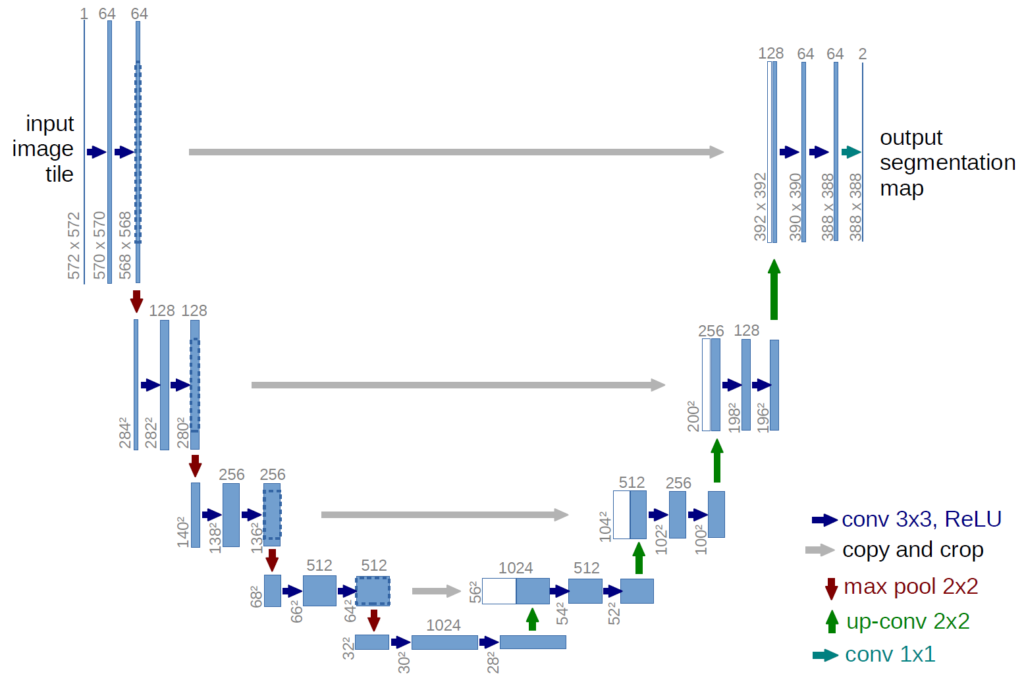
\includegraphics[width=0.8\linewidth]{PICTURES/unet-architecture.png}
    \caption{U-Net architecture \cite{ronneberger_u-net_2015}}
    \label{fig:unet-architecture}
\end{figure}

The input to a U-Net model is typically an image of size $H \times W \times C$, where $H$ is the height, $W$ is the width, and $C$ is the number of input channels. In Figure~\ref{fig:unet-architecture}, the input consists of grayscale images, where $C = 1$. For RGB images, $C = 3$. The output is an image of size $H \times W \times N$, where $N$ is the number of segmentation classes. In this case, there are two classes (binary segmentation), so $N = 2$.

\subsubsection{Upsampling with Transpose Convolutions}

The expanding path uses transpose convolutions (also called deconvolutions). Convolution reduces the image to a feature map, while transpose convolution upsamples the feature map back into an image.

\subsubsection{Skip Connections}

During the downsampling process, the network learns various features. However, as the feature maps shrink, details are lost. Skip connections allow the network to preserve these details by carrying them over from the earlier layers in the contracting path to the corresponding layers in the expanding path. This process helps retain important spatial information, improving segmentation accuracy. These connections are represented by the horizontal arrows in Figure~\ref{fig:unet-architecture}.
\subsubsection{Key Steps in U-Net Processing}
\begin{enumerate}
    \item In the contracting path, feature maps are progressively downsampled until the lowest resolution is reached.
    \item Before each downsampling step, feature maps are saved.
    \item During the upsampling process, saved feature maps are combined with the upsampled maps to recover spatial details \cite{ronneberger_u-net_2015}.
\end{enumerate}

\subsection{U-net and Microscopy}
A 2023 survey \cite{wu_state---art_2024} highlights U-Net as an effective model for microscopic image segmentation. This success is attributed to its ability to perform well with limited training data and its relatively quick training process. The survey also emphasizes the use of the original, unmodified U-Net, which has been widely applied in fields such as cytology and geology \cite{chen_deep_2020} (e.g., using scanning electron microscopy). Given that the images in this dataset share similar characteristics, the U-Net architecture is considered suitable for this task.

\subsection{Data Preprocessing – Augmentation}
The dataset consists of 150 training images, which are divided into training and validation subsets, along with 47 test images. To enhance the model's ability to generalize to unseen data, data augmentation is applied to train data.

The first step involves cropping the images to a predefined $n \times n$ size, where $n$ represents the patch size, a model hyperparameter. Cropping is done using the \textit{CropNonEmptyMaskIfExists}\cite{info11020125} function. This function ensures that the cropped region always contains parts of the coating, preserving important features. The cropping is applied with a probability of $p=1.0$, ensuring its occurrence.

Additional augmentations are applied with a probability of $p=0.3$ to increase variability. These include:

\begin{itemize}
    \item \textbf{Brightness and contrast adjustment:}This simulates lighting variations.
    \item \textbf{Sharpening:} This enhances the details in the image.
    \item \textbf{Horizontal flipping:} The image is mirrored along the horizontal axis to reduce positional bias.
    \item \textbf{Elastic transformation:} A non-linear deformation is applied to simulate distortions and improve generalization. It is applied with a probability of $p=0.5$.
\end{itemize}

The effects of these augmentations are illustrated in Figure \ref{fig:augmentation}, where different transformations are applied to a sample image.

\begin{figure}[H]
\centering
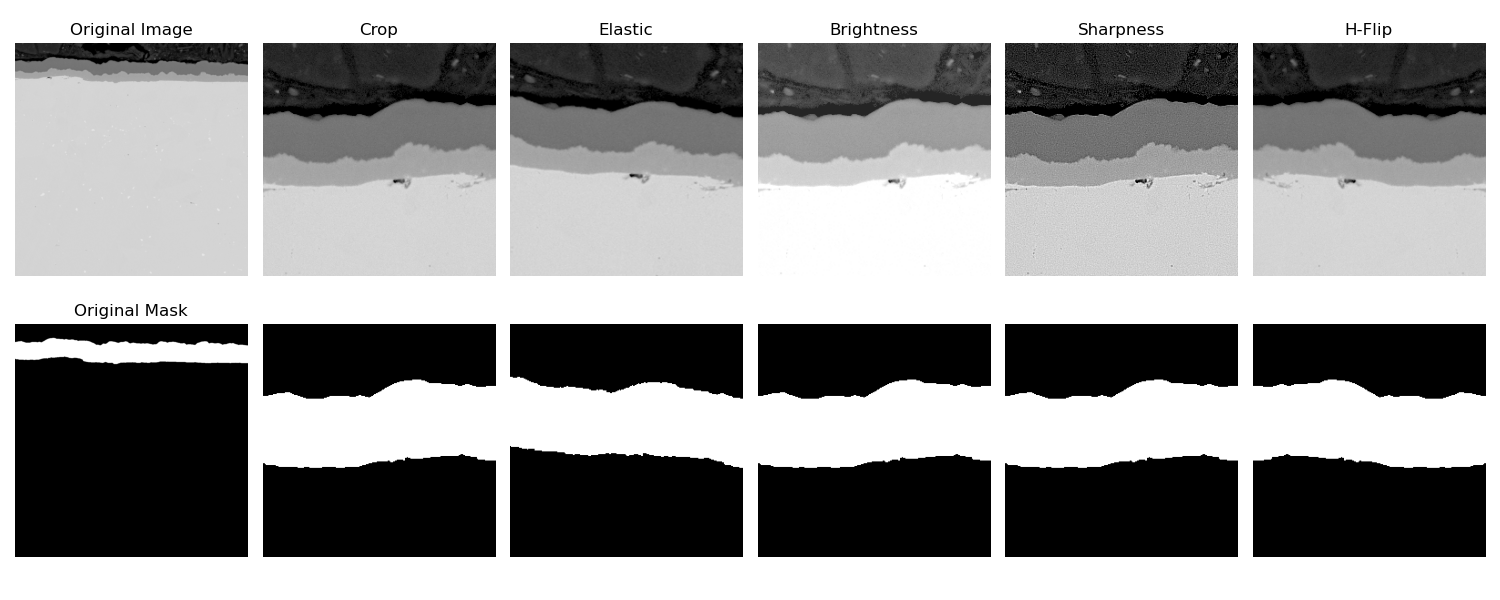
\includegraphics[width=1\linewidth]{PICTURES/augumentation.png}
\caption{Illustration of various augmentation techniques applied to the dataset.}
\label{fig:augmentation}
\end{figure}

\subsection{Technical Details}
The \texttt{segmentation\_models} library \cite{Iakubovskii:2019} was used for the U-Net implementation. Documentation for this implementation can be found \href{https://smp.readthedocs.io/en/latest/models.html#id21}{here} \cite{Iakubovskii_2019}. After initializing the training functions and other helper functions, hyperparameter tuning can begin. The main hyperparameters include depth, patch\_size, filters, and learning rates, all of which will be tested.

\subsection{Depth}
The depth of a U-Net is determined by the number of encoder and decoder blocks. This influences the model's ability to capture features within the input image. For instance, in Figure~\ref{fig:unet-architecture}, the depth is 5.

A deeper network (higher depth) can handle complex data with high variability, but may suffer from excessive downsampling and overfitting. In contrast, a shallower network may struggle to extract relevant features and differentiate between noise and useful information.

\subsection{Patch Size}
Patch size plays a crucial role in how well the model learns different features from the image.

Smaller patches allow the model to focus on fine details but might miss the broader context, making it harder to understand relationships between different parts of the image.

Larger patches capture more context and larger structures, but may lose fine details.

To ensure that the region of interest, specifically the coating layer, is always included, the images are cropped in a way that retains this key feature.

\subsection{Filters}
The filters parameter determines the number of filters used in each encoder and decoder layer, which affects the number of feature maps generated by the model. In the code, the number of filters in the decoder is calculated as follows:

\begin{verbatim}
decoder_channels = [filters * 2**i for i in range(depth, 0, -1)]
\end{verbatim}

This calculation, inspired by the original U-Net architecture, doubles the number of filters at each downsampling step \cite{2018arXiv180906839B}. For example, with \texttt{filters = 8} and \texttt{depth = 3}, the number of filters would be:  
\\\textbf{Encoder:} 8, 16, 32 \\
\textbf{Decoder:} 32, 16, 8

Using more filters allows the model to learn more complex patterns. However, it can also increase the risk of overfitting when there is insufficient training data. On the other hand, using fewer filters might prevent the model from capturing important features, reducing its performance.
\newpage
\subsection{Hyperparameter values}\label{sec:1.2.8}

In this project, all combinations of the following hyperparameters were tested:

\begin{itemize}
    \item \textbf{Patch size:} 128, 256
    \item \textbf{Depth:} 3, 4, 5
    \item \textbf{Filters:} 8, 16, 32
\end{itemize}

\subsection{Learning Rate and Schedulers}\label{sec:1.2.9}

During training, the model's parameters are adjusted to find the optimal solution. The \textbf{Adam optimizer} \cite{kingma2017adammethodstochasticoptimization} is used for this purpose. Adam (Adaptive Moment Estimation) calculates adaptive learning rates for each parameter.

Since Adam adapts the learning rate, manually modifying it can have a small impact but still affect performance. The learning rate is chosen from a range between 0 and the set value.

\begin{itemize}
    \item \textbf{Linear Scheduler:} The learning rate starts at the set value and decays linearly. The \textbf{end factor} multiplies the learning rate to finish at \textbf{end factor * lr}.
    \item \textbf{Warmup Cosine Scheduler:} The learning rate starts at a predefined value and decreases over \texttt{T\_0} epochs, following a cosine annealing schedule. After reaching the minimum, the learning rate resets and begins from the previous value, restarting the cycle.
\end{itemize}

The following schedulers and values were tested:
\begin{itemize}
    \item \textbf{LR values}: 0.01, 0.001, 0.0001
    \item \textbf{Linear scheduler}: With end factors of 0.01 and 0.001
    \item \textbf{Warmup Cosine scheduler}: With \texttt{T\_0}$= 25$ and \texttt{T\_0}$= 50$
\end{itemize}

Figure~\ref{fig:LRS} shows the learning rate schedulers. On the left, the linear scheduler spans 200 epochs, starting at 0.01 and ending at 0.001. On the right, the warmup cosine scheduler starts at 0.01 and ends at 0.00, with a warmup phase during the first 50 epochs.

\begin{figure}[H]
    \centering
    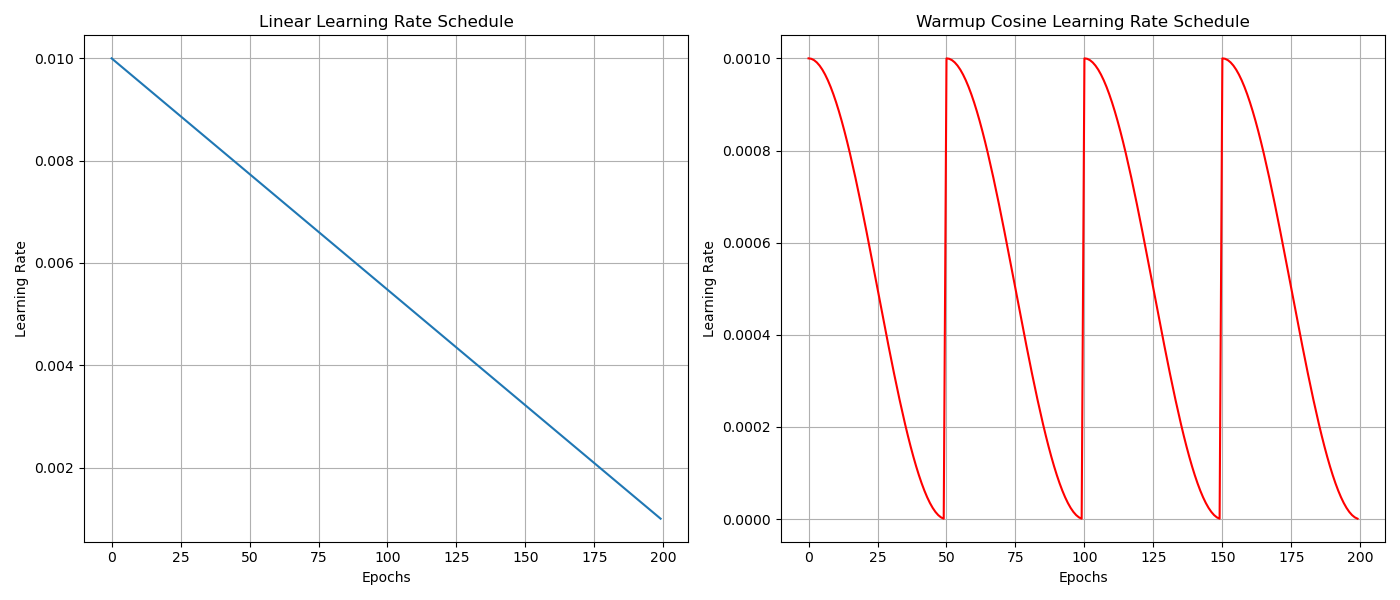
\includegraphics[width=0.9\linewidth]{PICTURES/LRS.png}
    \caption{Learning Rate Schedulers (LRS)}
    \label{fig:LRS}
\end{figure}
\subsection{Loss Function}

The loss function \( L(Y, \hat{Y}) \) is used to evaluate prediction errors. Since the model's performance on test data is assessed using the Intersection over Union (IoU) metric, IoU is also used as the loss function during training and validation.

The IoU is defined as:

\[
\text{IoU} = \frac{\text{intersection} + \text{smooth}}{\text{union} + \text{smooth}}
\]

Where:
\begin{itemize}
    \item The \( \text{intersection} \) is the number of pixels correctly predicted as the foreground (\(\text{True Positives}\)).
    \item The \( \text{union} \) consists of all pixels predicted or labeled as foreground. It equals the sum of \( \text{True Positives (TP)} \), \( \text{False Positives (FP)} \), and \( \text{False Negatives (FN)} \).
\end{itemize}

Thus, the IoU formula becomes:

\[
\text{IoU} = \frac{\text{TP} + \text{smooth}}{\text{TP} + \text{FP} + \text{FN} + \text{smooth}}
\]

The smoothing constant (\(\text{smooth} = 1\)) prevents division by zero. The loss function returns \( 1 - \text{IoU} \), ensuring that lower values indicate better model performance.

\subsection{Training}

After defining the key components, model training begins. The dataset is divided into 98 training images and 32 validation images. The training, validation, and testing labels come from the K-means refined dataset, with the validation set remaining fixed as a single batch.

During training, just the training data are shuffled each epoch to reduce the risk of overfitting. The shuffling function selects 32 random images for each batch. Training proceeds for either 200 or 150 epochs, with each epoch consisting of both training and validation phases.

\subsubsection{Training Phase}

In each epoch, the training dataset is shuffled, and three batches of 32 images are formed. The model predicts the binary mask for each batch and computes the training loss. Backpropagation adjusts the model's parameters using the optimizer based on the computed loss.

\subsubsection{Validation Phase}

At the end of each epoch, the validation set (a single batch) is evaluated using the loss function. The model's parameters are not updated during this phase. If the validation loss is lower than the previously recorded minimum, the model and its parameters are saved, and the minimum validation loss is updated.

\subsection{Optimization Strategy}

\begin{enumerate}
    \item Three optimization runs were performed to determine the optimal learning rate (LR) and learning rate scheduler. Details about the hyperparameters tested are provided in section \ref{sec:1.2.9}.
    \item The main optimization focused on the three key hyperparameters, using the best LR and LR scheduler from the initial optimization. The specific hyperparameters optimized are discussed in section \ref{sec:1.2.8}.
    \item After identifying the best hyperparameters, two additional runs were conducted. One used polygon labels, while the other used non-refined K-means labels.
\end{enumerate}
\subsection{Optimization results}

The optimization of the learning rate and learning rate schedulers is discussed first. The schedulers were tested with the hyperparameters \textbf{depth = 3}, \textbf{patch size = 128}, and \textbf{filters = 8}. These values were chosen as they offered the best computational efficiency among the tested ones. Initially, the warmup cosine scheduler was optimized. The contour plot below illustrates the relationship between \( T_0 \) and the learning rate. The optimal point occurs at \( T_0 = 50 \) and \( \text{lr} = 0.01 \), resulting in a minimum objective function value (IoU validation loss) of 0.03306.

\begin{figure}[H]
    \centering
    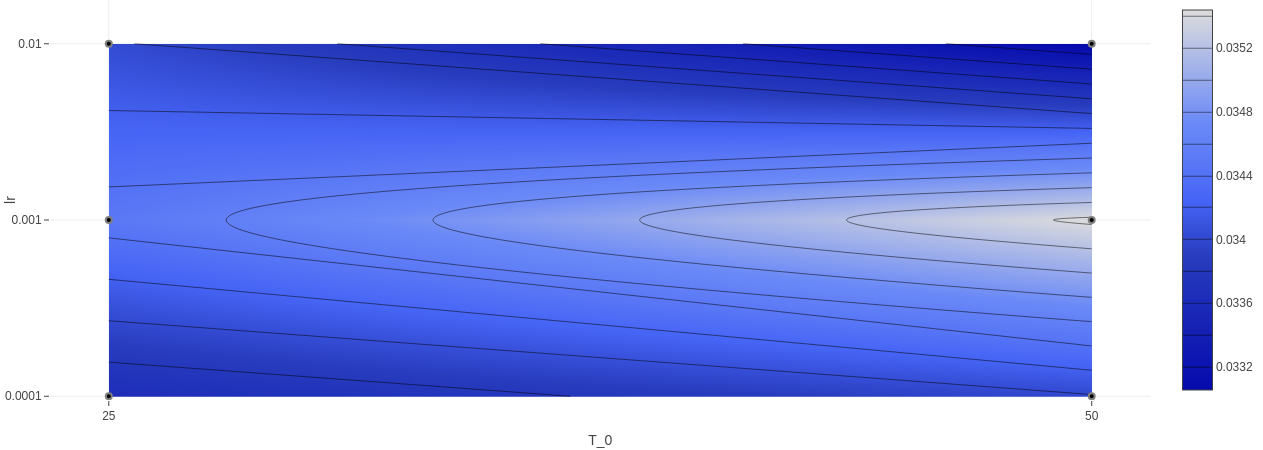
\includegraphics[width=0.75\linewidth]{PICTURES/cosine.png}
    \caption{Objective function contour: effect of \( T_0 \) and Learning Rate}
    \label{fig:cosine_contour}
\end{figure}

The best results for different learning rate schedulers are summarized in Table \ref{tab:scheduler_results}. The linear scheduler achieved the lowest objective function value of 0.03075 with a learning rate of 0.001 and an end factor of 0.001. The optimization without a scheduler resulted in a minimum objective function value of 0.03133 at a learning rate of 0.01.

\begin{table}[H]
    \centering
    \begin{tabular}{lccc}
        \toprule
        Schedule & Learning Rate (lr) & End Factor / \( T_0 \) & Val Loss \\
        \midrule
        Warmup Cosine & 0.01 & 50 & 0.03306 \\
        Linear & 0.001 & 0.001 & 0.03075 \\
        None & 0.01 & --- & 0.03133 \\
        \bottomrule
    \end{tabular}
    \caption{Best results for different Learning Rate Schedulers.}
    \label{tab:scheduler_results}
\end{table}

\newpage
Next, the main optimization was conducted using the linear scheduler and the best values from the previous step. The hyperparameters discussed in section \ref{sec:1.2.8} were optimized, resulting in 18 combinations (2 * 3 * 3 = 18). The complete results are shown in Table \ref{tab:main_results}, with the best result found at index 9.

\begin{table}[H]
\centering
\renewcommand{\arraystretch}{1}
\begin{tabular}{|c|c|c|c|c|}
\hline
\textbf{Idx} & \textbf{Val Loss} & \textbf{Depth} & \textbf{Filters} & \textbf{Patch Size} \\
\hline
0  & 0.03315 & 5  & 8   & 256 \\
1  & 0.03902 & 5  & 8   & 128 \\
2  & 0.03204 & 3  & 8   & 256 \\
3  & 0.03365 & 5  & 16  & 256 \\
4  & 0.02999 & 5  & 32  & 256 \\
5  & 0.03192 & 4  & 8   & 128 \\
6  & 0.03047 & 4  & 16  & 256 \\
7  & 0.03307 & 3  & 8   & 128 \\
8  & 0.03406 & 4  & 8   & 256 \\
\textbf{9}  & \textbf{0.02892} & \textbf{5}  & \textbf{16}  & \textbf{128} \\
10 & 0.03502 & 3  & 32  & 128 \\
11 & 0.03136 & 5  & 32  & 128 \\
12 & 0.03001 & 4  & 16  & 128 \\
13 & 0.02910 & 4  & 32  & 128 \\
14 & 0.03108 & 3  & 16  & 256 \\
15 & 0.03036 & 4  & 32  & 256 \\
16 & 0.03271 & 3  & 32  & 256 \\
17 & 0.03289 & 3  & 16  & 128 \\
\hline
\end{tabular}
\caption{Validation loss values with Depth, Filters, and Patch Size}
\label{tab:main_results}
\end{table}

Figure \ref{fig:validation_loss} presents the validation loss values over 150 epochs. Initially, both curves decrease rapidly, then oscillate around similar values, suggesting that the parameters no longer change significantly. The yellow line represents the best optimization, while the purple line represents the second-best optimization. From epoch 100 onward, the results stabilize. The optimization at index 9 provides the best performance. This model will be evaluated on the test dataset and implemented into the researcher's workflow.

\begin{figure}[H]
    \centering
    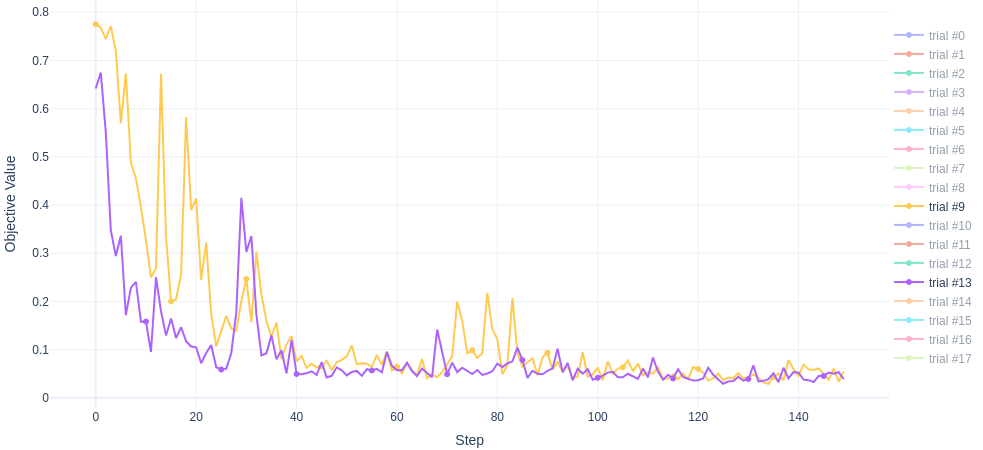
\includegraphics[width=0.75\linewidth]{PICTURES/lossFuncMain.png}
    \caption{Validation loss over 150 epochs}
    \label{fig:validation_loss}
\end{figure}

Additionally, Figure \ref{fig:Hyperparameter-Importance} shows the feature importances, indicating that patch size has the greatest impact on the results. This insight can be used in future work.

\begin{figure}[H]
    \centering
    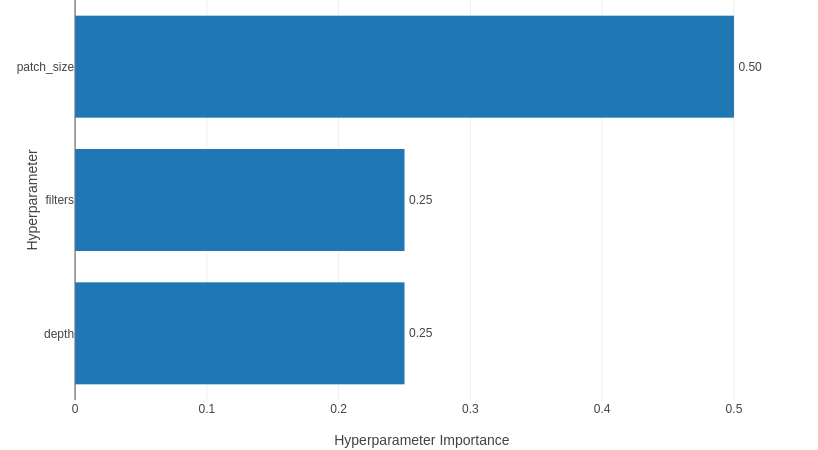
\includegraphics[width=0.75\linewidth]{PICTURES/importnace.png}
    \caption{Hyperparameter importance}
    \label{fig:Hyperparameter-Importance}
\end{figure}

The final two runs were conducted using the best hyperparameters, but with datasets that included labels generated by polygons and K-means clustering. The corresponding validation loss values are presented in Table \ref{tab:val_loss_values}.

\begin{table}[ht]
\centering
\renewcommand{\arraystretch}{1}
\begin{tabular}{|c|c|c|c|}
\hline
\textbf{Metric} & \textbf{K-means Refined} & \textbf{K-means} & \textbf{Polygon} \\
\hline
Validation Loss & 0.02892 & 0.03118 & 0.09698 \\
\hline
\end{tabular}
\caption{Validation loss values for different labeling methods}
\label{tab:val_loss_values}
\end{table}

Since both validation sets use labels from their respective training sets, these values may not be fully reliable. It is better to assess the model’s performance on unseen images using test labels generated from K-means refined clustering. Although the K-means and polygon labels are not intended for use in the final workflow, evaluating their performance on real test data could still provide useful insights.

\subsection{Evaluation on Test Data}

Two primary evaluation metrics were used:

\begin{itemize}
    \item \textbf{Mean IoU}: The intersection over union (IoU) is calculated and averaged across all test data.
    \item \textbf{Min IoU}: The minimum IoU value is used to assess the worst-case scenario.
\end{itemize}

The evaluation results are presented in Table \ref{tab:test_results}:

\begin{table}[ht]
\centering
\renewcommand{\arraystretch}{1.2}
\begin{tabular}{|c|c|c|c|}
\hline
\textbf{Metric} & \textbf{K-means Refined} & \textbf{K-means} & \textbf{Polygon} \\
\hline
Mean IoU & 0.95473 & 0.83111 & 0.92177 \\
Min IoU & 0.83872 & 0.17518 & 0.78456 \\
\hline
\end{tabular}
\caption{Evaluation Results on Test Data}
\label{tab:test_results}
\end{table}

The results reveal some key patterns. Although the "polygon" model was trained on validation data with polygon labels, it still performed well. This suggests that polygon labels could be used instead of K-means refined labels when applying the model to other parts of the images, such as various oxidation layers. They can also be used when retraining the model once more data is gathered. In such cases, K-means refinement may not be necessary, as polygon labels can be efficiently generated with a single script. On the other hand, the K-means labels without refinement performed poorly. This likely occurred because the model struggled to differentiate between oxidation and coating layers, which were not well-separated in the training data. In contrast, the K-means refined labels provided the best results on unseen data.

\newpage

\begin{figure}[H]
    \centering
    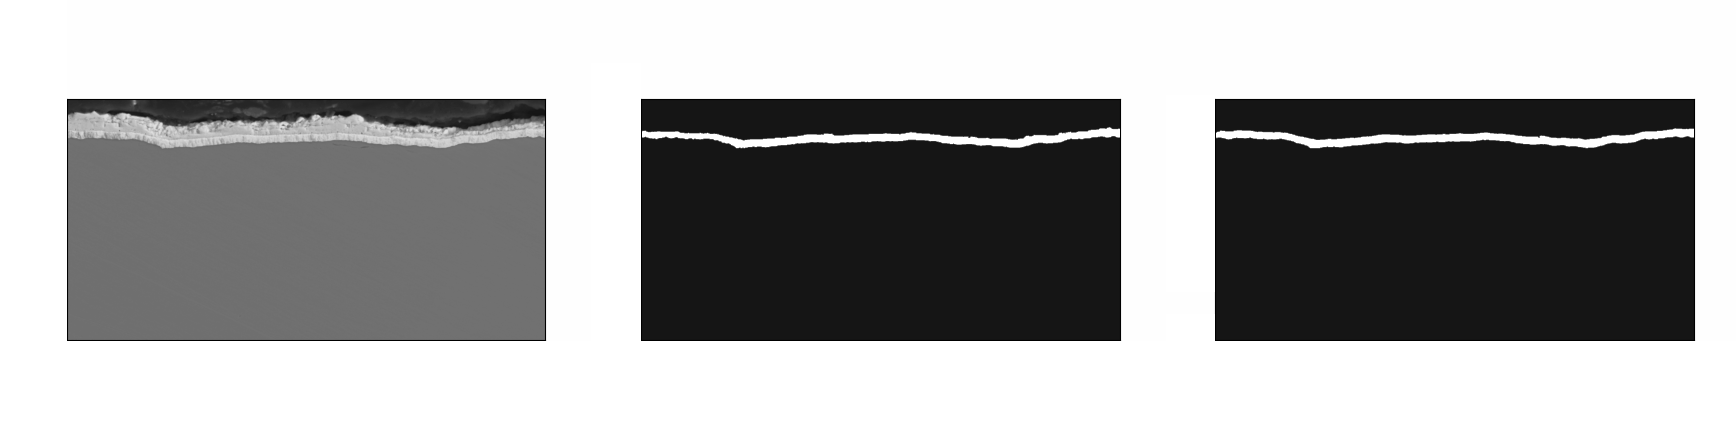
\includegraphics[width=1\linewidth]{PICTURES/refined_188_5_128_16_9.png}
    \caption{Original image, ground truth, prediction (K-means refined model)}
    \label{fig:refined_188_5_128_16_9}
\end{figure}

\begin{figure}[H]
    \centering
    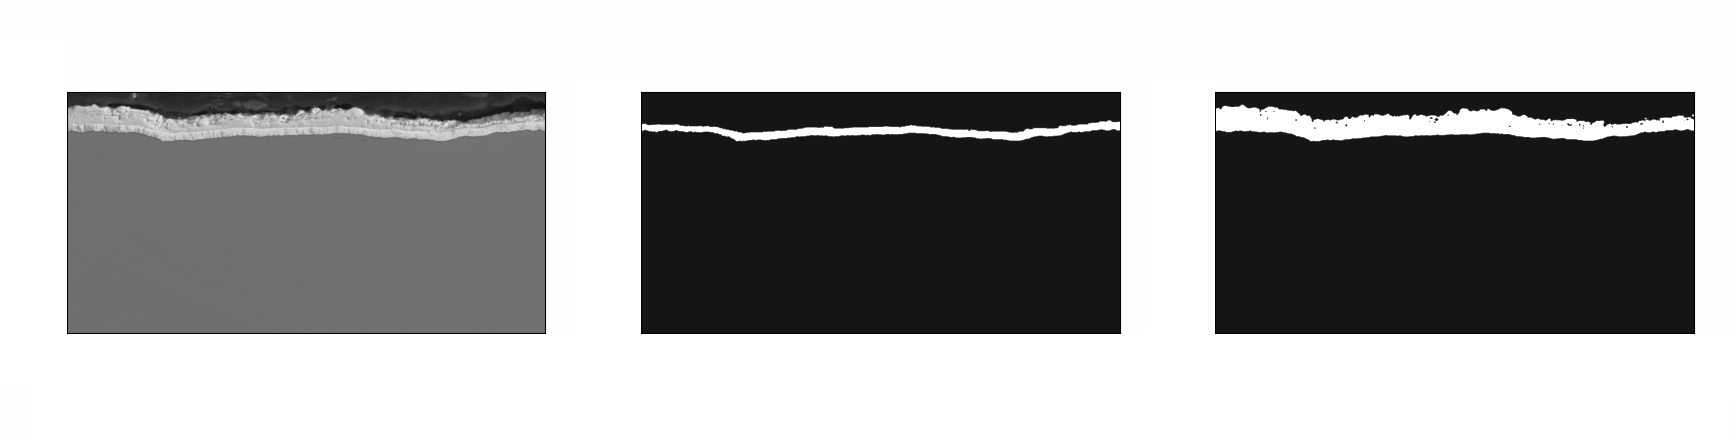
\includegraphics[width=1\linewidth]{PICTURES/kmeans_188_5_128_16_0.png}
    \caption{Original image, ground truth, prediction (K-means model)}
    \label{fig:kmeans_188_5_128_16_0}
\end{figure}

\begin{figure}[H]
    \centering
    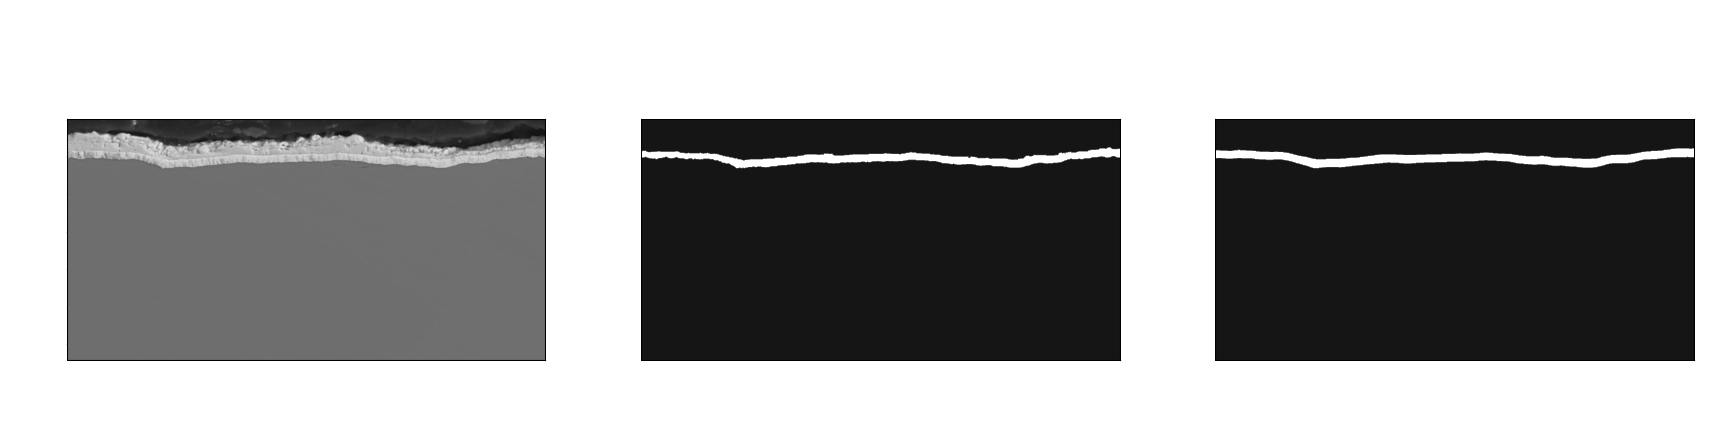
\includegraphics[width=1\linewidth]{PICTURES/polygon_188_5_128_16_0.png}
    \caption{Original image, ground truth, prediction (polygon model)}
    \label{fig:polygon_188_5_128_16_0}
\end{figure}

Figure \ref{fig:kmeans_188_5_128_16_0} illustrates that the model struggles to recognize the oxidation and coating layers, resulting in poor performance. In contrast, Figures \ref{fig:polygon_188_5_128_16_0} and \ref{fig:refined_188_5_128_16_9} demonstrate that the models can accurately predict coating layers, even though the images are complex and distinguishing between the layers is difficult.
